% SOAR Task Planner — System Architecture Diagram
% Compile with: pdflatex architecture_diagram.tex
% Requires: tikz, amsmath

\documentclass[tikz, border=16pt]{standalone}
\usepackage{tikz}
\usetikzlibrary{arrows.meta, fit, backgrounds, calc}
\usepackage{amsmath}

% ── Colour palette ─────────────────────────────────────────────────────────────
\definecolor{cBlue}  {RGB}{ 52, 152, 219}  % inputs
\definecolor{cOrange}{RGB}{230, 126,  34}  % instruction branch
\definecolor{cGreen} {RGB}{ 39, 174,  96}  % environmental branch
\definecolor{cPurple}{RGB}{155,  89, 182}  % joint CP
\definecolor{cTeal}  {RGB}{ 26, 188, 156}  % act path / output
\definecolor{cRed}   {RGB}{231,  76,  60}  % ask path
\definecolor{cDark}  {RGB}{ 52,  73,  94}  % understanding update
\definecolor{cGray}  {RGB}{127, 140, 141}  % human user

% ── Node width / height constants ─────────────────────────────────────────────
\newlength{\NW}\setlength{\NW}{4.0cm}
\newlength{\NH}\setlength{\NH}{0.82cm}

\begin{document}
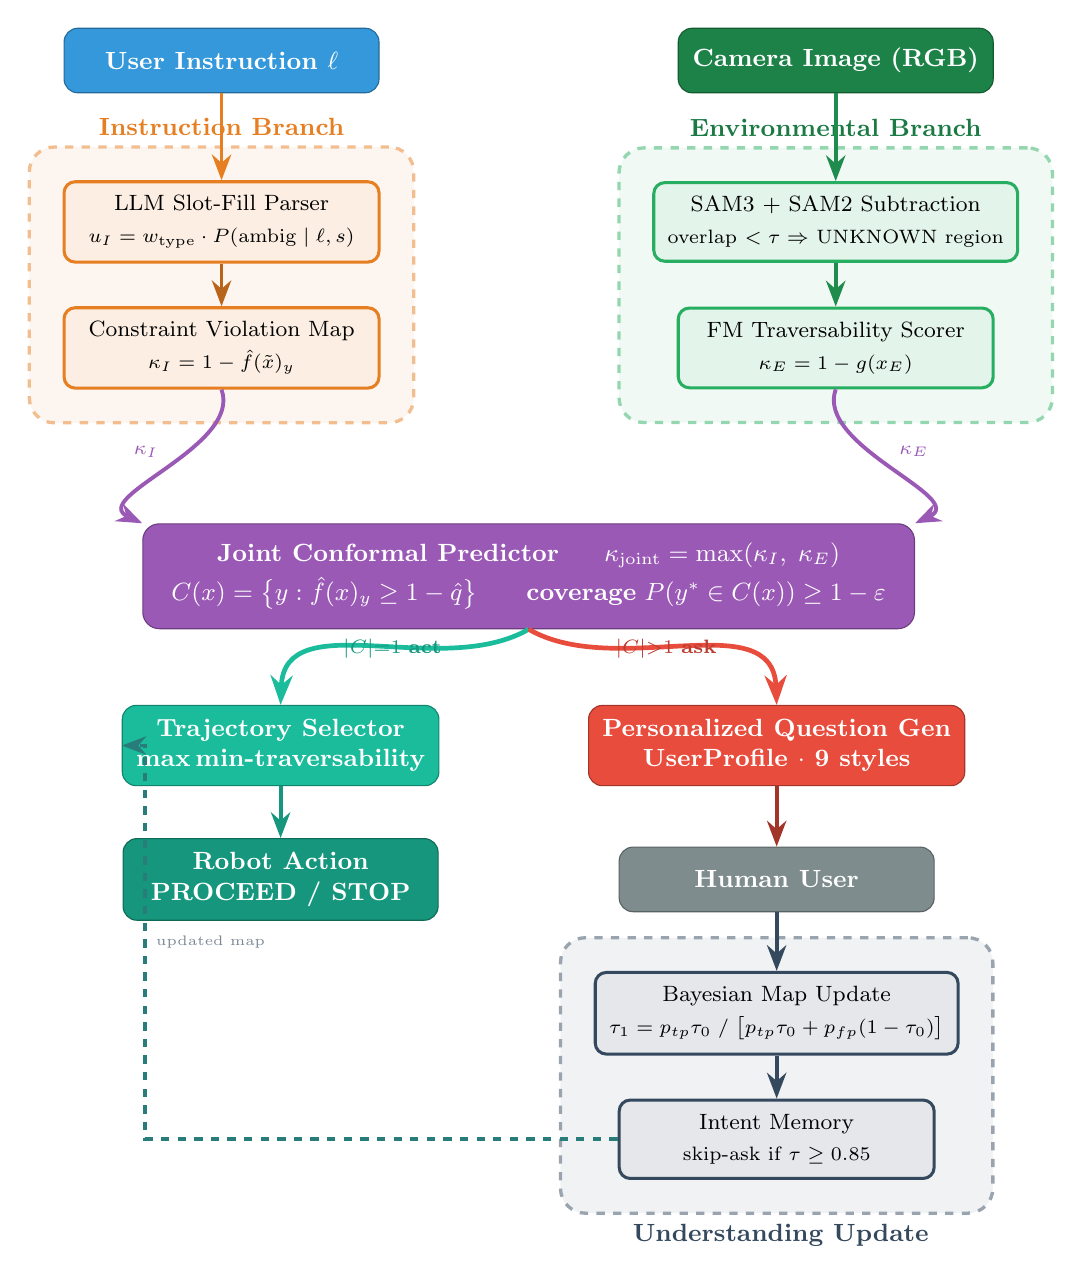
\begin{tikzpicture}[
  % ── Styles ──────────────────────────────────────────────────────────────────
  %
  % Solid filled input/output block (white text)
  inputN/.style args={#1}{
    rectangle, rounded corners=5pt,
    fill=#1, draw=#1!70!black, text=white,
    font=\small\bfseries,
    minimum width=\NW, minimum height=\NH,
    align=center, inner sep=5pt},
  %
  % Light-fill branch sub-block (coloured border)
  branchN/.style args={#1}{
    rectangle, rounded corners=4pt,
    fill=#1!13, draw=#1, line width=1.1pt, text=black,
    font=\footnotesize,
    minimum width=\NW, minimum height=\NH,
    align=center, inner sep=5pt},
  %
  % Wide solid block for joint CP
  cpN/.style={
    rectangle, rounded corners=6pt,
    fill=cPurple, draw=cPurple!70!black, text=white,
    font=\small\bfseries,
    minimum width=9.8cm, minimum height=1.2cm,
    align=center, inner sep=7pt},
  %
  % Solid path-decision blocks
  pathN/.style args={#1}{
    rectangle, rounded corners=5pt,
    fill=#1, draw=#1!70!black, text=white,
    font=\small\bfseries,
    minimum width=\NW, minimum height=\NH,
    align=center, inner sep=5pt},
  %
  % Dashed background box for grouped nodes
  bgN/.style args={#1}{
    rectangle, rounded corners=9pt,
    dashed, line width=1.2pt,
    draw=#1!50, fill=#1!7, inner sep=12pt},
  %
  % Arrow styles
  arr/.style args={#1}{-Stealth, line width=1.4pt, color=#1},
  arrW/.style args={#1}{-Stealth, line width=1.7pt, color=#1},
  arrD/.style args={#1}{-Stealth, line width=1.3pt, dashed, color=#1},
]

%% ════════════════════════════════════════════════════════════════════════════
%%  NODE LAYOUT
%%  Columns: instruction x=2.5, environmental x=10.3, CP centre x=6.4
%% ════════════════════════════════════════════════════════════════════════════

% ── Row 0: Inputs ─────────────────────────────────────────────────────────
\node[inputN=cBlue]          (instrIn)  at ( 2.5,   0) {User Instruction $\ell$};
\node[inputN=cGreen!75!black](camIn)    at (10.3,   0) {Camera Image (RGB)};

% ── Instruction branch (rows 1–2) ─────────────────────────────────────────
\node[branchN=cOrange]       (llmP)     at ( 2.5,  -2.05)
  {LLM Slot-Fill Parser\\[2pt]
   {\scriptsize $u_I = w_{\mathrm{type}} \cdot P(\mathrm{ambig} \mid \ell, s)$}};

\node[branchN=cOrange]       (conM)     at ( 2.5,  -3.65)
  {Constraint Violation Map\\[2pt]
   {\scriptsize $\kappa_I = 1 - \hat{f}(\tilde{x})_y$}};

% ── Environmental branch (rows 1–2) ───────────────────────────────────────
\node[branchN=cGreen]        (samD)     at (10.3,  -2.05)
  {SAM3 + SAM2 Subtraction\\[2pt]
   {\scriptsize overlap $< \tau \Rightarrow$ UNKNOWN region}};

\node[branchN=cGreen]        (fmS)      at (10.3,  -3.65)
  {FM Traversability Scorer\\[2pt]
   {\scriptsize $\kappa_E = 1 - g(x_E)$}};

% ── Row 3: Joint Conformal Predictor ──────────────────────────────────────
\node[cpN]                   (cpBox)    at ( 6.4,  -6.55)
  {Joint Conformal Predictor
   \hspace{1.2em}$\kappa_{\mathrm{joint}} = \max(\kappa_I,\;\kappa_E)$\\[3pt]
   {\small $C(x) = \bigl\{ y : \hat{f}(x)_y \geq 1-\hat{q} \bigr\}$
   \hspace{1em} coverage\;$P(y^* \in C(x)) \geq 1 - \varepsilon$}};

% ── Row 4: Act / Ask split ────────────────────────────────────────────────
\node[pathN=cTeal]           (trajSel)
  at ($(cpBox.center)+(-3.15,-2.15)$)
  {Trajectory Selector\\{\small max\,min-traversability}};

\node[pathN=cRed]            (qGen)
  at ($(cpBox.center)+( 3.15,-2.15)$)
  {Personalized Question Gen\\{\small UserProfile $\cdot$ 9 styles}};

% ── Row 5: Output / Human ─────────────────────────────────────────────────
\node[pathN=cTeal!80!black]  (robOut)
  at ($(trajSel.center)+(0,-1.7)$)
  {Robot Action\\PROCEED / STOP};

\node[inputN=cGray]          (human)
  at ($(qGen.center)+(0,-1.7)$)
  {Human User};

% ── Rows 6–7: Understanding Update ────────────────────────────────────────
\node[branchN=cDark]         (bayesU)
  at ($(human.center)+(0,-1.7)$)
  {Bayesian Map Update\\[2pt]
   {\scriptsize $\tau_1 = p_{tp}\tau_0 \;/\;
   \bigl[p_{tp}\tau_0 + p_{fp}(1-\tau_0)\bigr]$}};

\node[branchN=cDark]         (intentM)
  at ($(bayesU.center)+(0,-1.6)$)
  {Intent Memory\\[2pt]
   {\scriptsize skip-ask if $\tau \geq 0.85$}};


%% ════════════════════════════════════════════════════════════════════════════
%%  ARROWS
%% ════════════════════════════════════════════════════════════════════════════

% Inputs → branches
\draw[arr=cOrange]           (instrIn) -- (llmP);
\draw[arr=cGreen!80!black]   (camIn)   -- (samD);

% Within branches
\draw[arr=cOrange!80!black]  (llmP)    -- (conM);
\draw[arr=cGreen!80!black]   (samD)    -- (fmS);

% κ_I, κ_E → Joint CP (curved, converging from each branch)
\draw[arr=cPurple]
  (conM.south)
  to[out=-70, in=155]
  node[midway, above left, font=\scriptsize\bfseries, text=cPurple] {$\kappa_I$}
  (cpBox.north west);

\draw[arr=cPurple]
  (fmS.south)
  to[out=-110, in=25]
  node[midway, above right, font=\scriptsize\bfseries, text=cPurple] {$\kappa_E$}
  (cpBox.north east);

% Joint CP → Act (|C|=1) and Ask (|C|>1) paths
\draw[arrW=cTeal]
  (cpBox.south)
  to[out=-150, in=88]
  node[near start, left, font=\scriptsize\bfseries, text=cTeal!80!black]
    {$|C|{=}1$\;act}
  (trajSel.north);

\draw[arrW=cRed]
  (cpBox.south)
  to[out=-30, in=92]
  node[near start, right, font=\scriptsize\bfseries, text=cRed!80!black]
    {$|C|{>}1$\;ask}
  (qGen.north);

% Act path downward
\draw[arr=cTeal!80!black]    (trajSel) -- (robOut);

% Ask path downward
\draw[arr=cRed!70!black]     (qGen)    -- (human);
\draw[arr=cDark]             (human)   -- (bayesU);
\draw[arr=cDark]             (bayesU)  -- (intentM);

% Feedback: updated map + intent → trajectory selector (wide dashed arc)
\draw[arrD=cDark!55!cTeal]
  (intentM.west)
  -- ++(-6.0, 0)
  coordinate (feedCorner)
  -- (feedCorner |- trajSel.west)
  node[midway, right, font=\tiny, text=cDark!65] {updated map}
  -- (trajSel.west);


%% ════════════════════════════════════════════════════════════════════════════
%%  BACKGROUND BRANCH BOXES
%% ════════════════════════════════════════════════════════════════════════════
\begin{scope}[on background layer]
  \node[bgN=cOrange,
        fit=(llmP)(conM),
        label={[text=cOrange, font=\small\bfseries]above:Instruction Branch}]
        (instrBG) {};

  \node[bgN=cGreen,
        fit=(samD)(fmS),
        label={[text=cGreen!70!black, font=\small\bfseries]above:Environmental Branch}]
        (envBG) {};

  \node[bgN=cDark,
        fit=(bayesU)(intentM),
        label={[text=cDark, font=\small\bfseries]below:\;Understanding Update}]
        (updBG) {};
\end{scope}

\end{tikzpicture}
\end{document}
